% Asal-usul (tidak pernah dicetak): lihat sources/outline_sources.md (Tahun 1: pelapukan fisik dan kimia; hidrolisis dan derajatnya; diagram potensial ionik; mineral lempung dan iklim; pelapukan silikat dan karbon dioksida). Nilai soal latihan dan soal dari kalkulator skrap Buku 3 calc/ch19.py; data gambar dari figdata/bachelor-1/ionic_potential.py dan hydrolysis.py. Pelapukan dimiliki oleh Buku 1 kelas 5; pelapukan kimia, hidrolisis, mineral lempung dan laterit oleh Buku 2 kelas 10 (dibangun ulang di sini). Kelas silikat dan feldspar oleh bab 7; deret reaksi Bowen oleh Buku 2 kelas 11; kimia asam--basa, kelarutan dan oksidasi oleh buku-buku kimia; tanah dan horizonnya oleh buku-buku biologi. Termostat pelapukan silikat termasuk dalam volume Tahun ke-2 (diceritakan).
\chapter{Pelapukan dan lempung}\label{ch:b1:weathering-clays}

Huruf-huruf pada batu nisan tua memudar, tepi-tepi tajamnya membulat menjadi alur dangkal, lebih cepat pada batu marmer daripada pada batu sabak. \omterm{def:b1:geological-maps:geological-map}{Singkapan} granit yang tampak sekeras apa pun di Bumi hancur di permukaannya menjadi pasir kasar, yang mengalir di sela jari sebagai butiran lepas kuarsa berkilau, \omterm{def:b1:rock-forming-minerals:groups}{feldspar} kapur dan serpihan \omterm{def:b1:rock-forming-minerals:groups}{mika}. Di bawah hutan tropis yang lembap, batuan padat mungkin terletak jauh di bawah, di bawah tanah merah yang masih mempertahankan garis-garis \omterm{def:b1:rock-forming-minerals:mineral}{mineral} batuan tetapi dapat dipotong dengan sekop. Ketiganya adalah hasil kerja air di permukaan Bumi. Bab ini menuliskan kerja itu sebagai kimia: \omterm{def:b1:rock-forming-minerals:mineral}{mineral} mana yang menyerah lebih dulu, apa yang mereka menjadi, mengapa sebagian unsur pergi bersama air dan yang lain tinggal, bagaimana iklim menentukan hasilnya, dan bagaimana pelapukan lambat batuan silikat menarik karbon dioksida keluar dari udara.

\begin{recall}
Pelapukan memecah batuan di tempat ia berada (Buku 1, kelas 5). \omterm{def:b1:weathering-clays:weathering}{Pelapukan kimia} mengubah \omterm{def:b1:rock-forming-minerals:mineral}{mineral}; \omterm{def:b1:weathering-clays:hydrolysis}{hidrolisis} \omterm{def:b1:rock-forming-minerals:groups}{feldspar} menghasilkan \omterm{def:b1:weathering-clays:clay-mineral}{mineral lempung}, \omterm{def:b1:weathering-clays:clay-mineral}{kaolinit}, dan mengirim kalium dan silika ke sungai; \omterm{def:b1:weathering-clays:laterite}{laterit} adalah produk merah yang kaya besi dan aluminium dari iklim panas dan basah (Buku 2, kelas 10). Silikat diklasifikasikan menurut cara tetrahedra \ce{SiO4} berbagi sudut, fillosilikat membentuk lembaran; \omterm{def:b1:rock-forming-minerals:groups}{feldspar} adalah silikat kerangka natrium, kalium dan kalsium, \omterm{def:b1:rock-forming-minerals:groups}{mika} silikat lembaran dengan kalium di antara lembaran (\cref{def:b1:rock-forming-minerals:silicate-classes}, \cref{def:b1:rock-forming-minerals:groups}). Radius ion bergantung pada muatannya dan koordinasinya (\cref{ch:b1:rock-forming-minerals}). \omterm{def:b1:rock-forming-minerals:mineral}{Mineral} mengkristal dari magma yang mendingin dalam urutan deret reaksi Bowen, \omterm{def:b1:rock-forming-minerals:groups}{olivin} pertama dan kuarsa terakhir (Buku 2, kelas 11). Asam melepaskan ion hidrogen; karbon dioksida yang larut dalam air membentuk asam karbonat; oksidasi adalah kehilangan elektron; persamaan yang seimbang menjaga setiap unsur dan muatan (buku-buku kimia). Tanah adalah lapisan hidup yang tersusun dalam horizon (buku-buku biologi).
\end{recall}

\section{Pelapukan fisik dan kimia}\label{sec:b1:weathering-clays:types}

Batuan yang terbentuk di kedalaman, pada suhu dan tekanan tinggi dan tanpa air bebas atau oksigen, berada di luar kesetimbangan di permukaan. Ia menyesuaikan diri dengan dua cara, yang bekerja bersama.

\begin{definition}[Pelapukan fisik, pelapukan kimia]\label{def:b1:weathering-clays:weathering}
\emph{Pelapukan fisik}\index{pelapukan fisik} adalah pemecahan batuan di tempatnya menjadi fragmen-fragmen yang lebih kecil tanpa perubahan \omterm{def:b1:rock-forming-minerals:mineral}{mineralnya}. \emph{Pelapukan kimia}\index{pelapukan kimia} adalah transformasi \omterm{def:b1:rock-forming-minerals:mineral}{mineral} suatu batuan di tempatnya oleh reaksi dengan air dan zat-zat yang dibawanya, terutama ion hidrogen, karbon dioksida terlarut dan oksigen: sebagian \omterm{def:b1:rock-forming-minerals:mineral}{mineral} larut, yang lain digantikan oleh \omterm{def:b1:rock-forming-minerals:mineral}{mineral} baru yang stabil di permukaan, dan sebagian batuan pergi dalam larutan.
\end{definition}
% ledger: formoso:weathering

\emph{Beku.} Air pada \qty{0}{\celsius} memiliki massa jenis \qty{999.87}{kg.m^{-3}}, es \qty{916.72}{kg.m^{-3}}: air memuai sebesar \qty{9.1}{\percent} saat membeku. Gambaran lama pelapukan beku adalah air yang membeku dalam retakan tertutup dan memaksanya terbuka, lagi pada setiap pencairan dan pembekuan. Model retakan pada granit dan marmer, dibangun di atas mekanika rekahan dan apa yang diketahui tentang tanah beku, menempatkan bebannya di tempat lain: air ditarik melalui pori-pori menuju es yang sudah ada di dalam retakan, seperti halnya menuju lensa es dalam tanah beku, dan es tumbuh serta menyelipi retakan selama pembekuan berlangsung. Pembekuan yang bertahan paling efektif antara sekitar \qty{-4}{\celsius} dan \qty{-15}{\celsius}: lebih dekat ke nol es tidak dapat membangun tekanan yang cukup, dan lebih dingin air tidak lagi dapat bergerak menuju es itu.
% ledger: usgs:water-density, iapws:ice-density, wh85:frost

\emph{Pemanasan, pembebasan beban dan garam.} Pemanasan dan pendinginan berulang melelahkan batuan yang \omterm{def:b1:rock-forming-minerals:mineral}{mineral-mineralnya} memuai dengan besar yang berbeda; granit yang dibawa ke permukaan oleh erosi, terlepas dari beban di atasnya, memuai dan pecah menjadi lembaran-lembaran sejajar permukaan; garam yang mengkristal dari air yang menguap, di gurun dan di pantai, mencongkel butiran-butiran terpisah.

\omterm{def:b1:weathering-clays:weathering}{Pelapukan fisik} lebih dari sekadar memecah batuan: ia membukanya bagi air.

\begin{proposition}[Permukaan yang terbuka oleh fragmentasi]\label{prop:b1:weathering-clays:surface}
Sebuah kubus bersisi $L$ yang dipotong menjadi kubus-kubus bersisi $L/n$ memiliki luas permukaan $n$ kali lebih besar. Lebih umum, massa $m$ butiran dengan massa jenis $\rho$, semuanya kubus bersisi $d$, memiliki luas permukaan $S = 6m/(\rho d)$: permukaan spesifik $S/m =
6/(\rho d)$ berbanding terbalik dengan ukuran butir.
\end{proposition}

\begin{proof}
Sebuah kubus bersisi $d$ memiliki luas $6d^2$ dan massa $\rho d^3$, sehingga permukaan spesifik setiap butir, dan sejumlah berapa pun dari mereka, adalah $6d^2/(\rho d^3)
= 6/(\rho d)$. Memotong kubus bersisi $L$ menjadi $n^3$ kubus bersisi $L/n$ mempertahankan massa dan membagi $d$ dengan $n$, yang melipatgandakan luas sebanyak $n$ kali.
\end{proof}

Blok \omterm{def:b1:rock-forming-minerals:groups}{feldspar} dengan massa jenis sekitar \qty{2600}{kg.m^{-3}} memiliki permukaan spesifik \qty{0.23}{m^2.kg^{-1}} sebagai fragmen sentimeter, dan \qty{2.3}{m^2.g^{-1}} sebagai butir mikrometer, sepuluh ribu kali lebih banyak. Reaksi kimia berlangsung di permukaan, sehingga batuan yang dihancurkan oleh beku atau terbuka sepanjang sambungannya melapuk secara kimia jauh lebih cepat daripada batuan yang sama yang masih utuh.
% ledger: hom:albite, hom:orthoclase

\emph{Reaksi-reaksi kimianya.} Kalsit larut sepenuhnya dalam air yang membawa karbon dioksida, itulah sebabnya nisan marmer kehilangan hurufnya (Buku~2, kelas~10). Besi(II) dari silikat gelap teroksidasi menjadi besi(III), yang tetap sebagai oksida kuning-cokelat dan merah. Yang paling penting, karena silikat membentuk sebagian besar \omterm{def:b1:layered-earth:layers}{kerak}, adalah \omterm{def:b1:weathering-clays:hydrolysis}{hidrolisis}. Ion hidrogen berasal dari karbon dioksida, yang larut dari udara dan dihembuskan oleh akar serta pengurai ke dalam tanah, dan dari asam organik tumbuhan yang membusuk: air permukaan dan air tanah yang tidak tercemar memiliki pH antara 5.5 dan 7, dan air lapisan organik beberapa tanah hutan bahkan serendah 3.5. Air, suhu, luas permukaan dan keasaman dengan demikian adalah empat pengendali \omterm{def:b1:weathering-clays:weathering}{pelapukan kimia}, dan iklim hangat dan basah dengan tanah tebal menyediakan keempatnya.
% ledger: formoso:weathering

\section{Hidrolisis silikat}\label{sec:b1:weathering-clays:hydrolysis}

\begin{definition}[Hidrolisis silikat]\label{def:b1:weathering-clays:hydrolysis}
\emph{Hidrolisis}\index{hidrolisis (silikat)} suatu silikat adalah reaksinya dengan air dan ion hidrogen, di mana ion hidrogen menggantikan kation logam, yang masuk ke dalam larutan; sebagian atau seluruh silikon keluar sebagai asam silikat terlarut \ce{H4SiO4}, dan sisa \omterm{def:b1:rock-forming-minerals:mineral}{mineral} dibangun kembali menjadi padatan baru, \omterm{def:b1:weathering-clays:clay-mineral}{mineral lempung} atau hidroksida. Pelarutannya tidak kongruen: padatan yang tersisa tidak memiliki komposisi \omterm{def:b1:rock-forming-minerals:mineral}{mineral} yang diserang.
\end{definition}
% ledger: formoso:weathering

Aluminium adalah kunci untuk menuliskan reaksinya: pada pH tanah dan sungai ia hampir tidak larut, dan produk padat menyimpan seluruhnya. Semua yang lain mengikuti dari situ.

\begin{method}[Menyeimbangkan reaksi hidrolisis]\label{met:b1:weathering-clays:balance}
Diberikan \omterm{def:b1:rock-forming-minerals:mineral}{mineral} yang diserang dan produk padatnya:
\begin{enumerate}
  \item Ambil satu satuan rumus produk, dan sebanyak \omterm{def:b1:rock-forming-minerals:mineral}{mineral} yang membawa jumlah atom aluminium yang sama.
  \item Silikon \omterm{def:b1:rock-forming-minerals:mineral}{mineral} yang tidak digunakan oleh produk keluar sebagai \ce{H4SiO4}; kation logam yang tidak digunakan oleh produk keluar sebagai ion.
  \item Seimbangkan muatan kation ini dengan ion hidrogen di ruas kiri.
  \item Seimbangkan oksigen dengan air di ruas kiri.
  \item Periksa hidrogen: ia harus seimbang dengan sendirinya. Jika tidak, ada rumus yang salah.
  \item Jika persamaan bilangan bulat diinginkan, kalikan seluruhnya.
\end{enumerate}
\end{method}

\begin{proposition}[Hidrolisis feldspar]\label{prop:b1:weathering-clays:feldspars}
Dengan \omterm{def:b1:weathering-clays:clay-mineral}{smektit} beidelit \ce{Na_{0.5}Al2(Si_{3.5}Al_{0.5})O10(OH)2}
(air antarlapisan tidak disertakan), \omterm{def:b1:weathering-clays:clay-mineral}{kaolinit} \ce{Al2Si2O5(OH)4} dan gibsit
\ce{Al(OH)3} sebagai produk,
\begin{align*}
&\ce{5 NaAlSi3O8 + 4 H+ + 16 H2O -> 2 Na_{0.5}Al2(Si_{3.5}Al_{0.5})O10(OH)2 + 4 Na+ + 8 H4SiO4},\\ % ce-unbalanced-ok: decimal subscripts the checker cannot read; balance tested in tests/bachelor-1/test_weathering_clays.py
&\ce{2 NaAlSi3O8 + 2 H+ + 9 H2O -> Al2Si2O5(OH)4 + 2 Na+ + 4 H4SiO4},\\
&\ce{NaAlSi3O8 + H+ + 7 H2O -> Al(OH)3 + Na+ + 3 H4SiO4},\\
&\ce{CaAl2Si2O8 + 2 H+ + H2O -> Al2Si2O5(OH)4 + Ca^2+}.
\end{align*}
Albit kehilangan \qty{80}{\percent} natriumnya dan $8/15$ silikonnya ke dalam larutan pada reaksi pertama, seluruh natriumnya dan $2/3$ silikonnya pada reaksi kedua, seluruh keduanya pada reaksi ketiga. Anortit kehilangan seluruh kalsiumnya dan tidak ada silikonnya sama sekali.
\end{proposition}
% ledger: webmineral:clays-b19, hom:albite, hom:anorthite

\begin{proof}
Terapkan metodenya. Reaksi pertama: dua satuan beidelit memegang $2\times2.5 = 5$ aluminium, yaitu aluminium dari 5 albit; 15 silikon albit dikurangi $2\times3.5 = 7$ dari produk menyisakan 8 \ce{H4SiO4}; 5 natrium dikurangi 1 menyisakan 4 \ce{Na+}, diseimbangkan oleh 4 \ce{H+}; oksigen, $40 + w$ di ruas kiri dan $24 + 32 =
56$ di ruas kanan, memberi $w = 16$; hidrogen, $4 + 32 = 36$ dan $4 + 32 = 36$, cocok. Kedua: 2 albit memberi 2 aluminium \omterm{def:b1:weathering-clays:clay-mineral}{kaolinit}, $6 - 2 = 4$ \ce{H4SiO4}, 2 \ce{Na+} dan 2 \ce{H+}; oksigen $16 + w = 9 + 16$ memberi $w = 9$; hidrogen $2 + 18 = 20 = 4 + 16$. Ketiga: satu albit, tiga asam silikat, satu \ce{Na+} dan satu \ce{H+}; oksigen $8 + w = 3 + 12$ memberi $w = 7$; hidrogen $1 + 14 = 15 = 3 + 12$. Keempat: 2 aluminium dan 2 silikon anortit persis sama dengan yang ada pada \omterm{def:b1:weathering-clays:clay-mineral}{kaolinit}, tidak ada asam silikat yang keluar, \ce{Ca^2+} membutuhkan 2 \ce{H+}; oksigen $8 + w = 9$ memberi $w = 1$; hidrogen $2 + 2 = 4$. Pecahan yang diekspor adalah jumlah ion dalam larutan dibagi jumlah atom dalam \omterm{def:b1:rock-forming-minerals:mineral}{mineral}: $4/5$ dan $8/15$, lalu $2/2$ dan $4/6$, lalu $1/1$ dan $3/3$.
\end{proof}

Albit yang sama dengan demikian dapat menghasilkan tiga padatan yang berbeda, dan padatan mana yang terbentuk bergantung pada seberapa banyak air yang melewati batuan dan membawa produknya pergi: sedikit air, dan banyak silika serta sebagian kation tetap tinggal untuk membangun \omterm{def:b1:weathering-clays:clay-mineral}{smektit}; lebih banyak, dan hanya cukup silika untuk \omterm{def:b1:weathering-clays:clay-mineral}{kaolinit} yang tersisa; sangat banyak, dan silika keluar seluruhnya.

\begin{definition}[Bisiallitisasi, monosiallitisasi, alitisasi]\label{def:b1:weathering-clays:hydrolysis-degree}
Derajat \omterm{def:b1:weathering-clays:hydrolysis}{hidrolisis} silikat dinamai menurut produknya. \emph{Bisiallitisasi}\index{bisiallitisasi} membentuk \omterm{def:b1:weathering-clays:clay-mineral}{mineral lempung} 2:1, seperti \omterm{def:b1:weathering-clays:clay-mineral}{smektit}, dengan sekitar dua atom silikon per aluminium; sebagian kation tetap berada di dalamnya. \emph{Monosiallitisasi}\index{monosiallitisasi} membentuk \omterm{def:b1:weathering-clays:clay-mineral}{mineral lempung} 1:1, \omterm{def:b1:weathering-clays:clay-mineral}{kaolinit}, dengan satu silikon per aluminium; semua kation \omterm{def:b1:rock-forming-minerals:groups}{alkali} dan alkali-tanah keluar. \emph{Alitisasi}\index{alitisasi} menghilangkan silikon seluruhnya dan menyisakan aluminium hidroksida, gibsit.
\end{definition}
% ledger: pedron:stages, formoso:weathering

Derajat yang tercapai terutama ditentukan oleh iklim, lewat curah hujan dan suhu, lalu oleh drainase profil. Di tempat air sedikit diperbarui, granit kehilangan banyak natrium dan kalsiumnya, kalium lebih lambat, dan hanya sebagian silikanya: \omterm{def:b1:rock-forming-minerals:groups}{feldsparnya} berubah menjadi lempung 2:1, dan banyak kuarsa tersisa; batuan itu pecah menjadi pasir kuarsa, \omterm{def:b1:rock-forming-minerals:groups}{mika} dan \omterm{def:b1:rock-forming-minerals:groups}{feldspar} setengah lapuk yang bercampur dengan lempung. Di bawah hujan lebat di tropika lembap, lebih dari \qty{2000}{mm} setahun, kation dan silika tercuci jauh lebih banyak, dan terbentuklah \omterm{def:b1:weathering-clays:clay-mineral}{kaolinit}, Si/Al = 1. Di tempat pencucian paling intens, bahkan silika \omterm{def:b1:weathering-clays:clay-mineral}{kaolinit} pun hilang, dan gibsit tersisa.
% ledger: pedron:stages, goldich:1938, formoso:laterite

\begin{omfigure}
\begin{tikzpicture}[font=\small]
% fractions of albite's Na and Si exported by the three degrees (figdata/bachelor-1/hydrolysis.py)
\begin{axis}[width=10.5cm, height=6cm, ybar, bar width=0.5cm, ymin=0, ymax=112,
    xmin=0.45, xmax=3.55, xtick={1,2,3},
  xticklabels={{bisiallitisasi\\ ke beidelit\\ (Si/Al = 1.4)}, {monosiallitisasi\\ ke kaolinit\\ (Si/Al = 1)}, {alitisasi\\ ke gibsit\\ (Si/Al = 0)}},
    xticklabel style={align=center, font=\footnotesize},
    ylabel={diekspor dalam larutan (\si{\percent})}, ytick={0,20,...,100},
    legend style={at={(0.5,1.03)}, anchor=south, font=\footnotesize, legend columns=2, draw=none},
    nodes near coords={\pgfmathprintnumber[fixed,precision=0]{\pgfplotspointmeta}}, every node near coord/.append style={font=\scriptsize},
    enlarge x limits=false]
  \addplot[fill=omThm!60, draw=omThm!80!black] table[x=degree, y=Na] {figdata/out/bachelor-1-hydrolysis-degrees.dat};
  \addplot[fill=omDef!55, draw=omDef!80!black] table[x=degree, y=Si] {figdata/out/bachelor-1-hydrolysis-degrees.dat};
  \legend{natrium, silikon}
\end{axis}
\end{tikzpicture}

{\small Tiga derajat \omterm{def:b1:weathering-clays:hydrolysis}{hidrolisis} albit: persentase natrium dan silikonnya yang terbawa pergi dalam larutan, dihitung dari reaksi-reaksi yang seimbang, serta rasio silikon terhadap aluminium pada padatan yang tersisa. Aluminium tetap seluruhnya di dalam padatan pada ketiganya.}
\label{fig:b1:weathering-clays:degrees}
\end{omfigure}


\begin{omfigure}
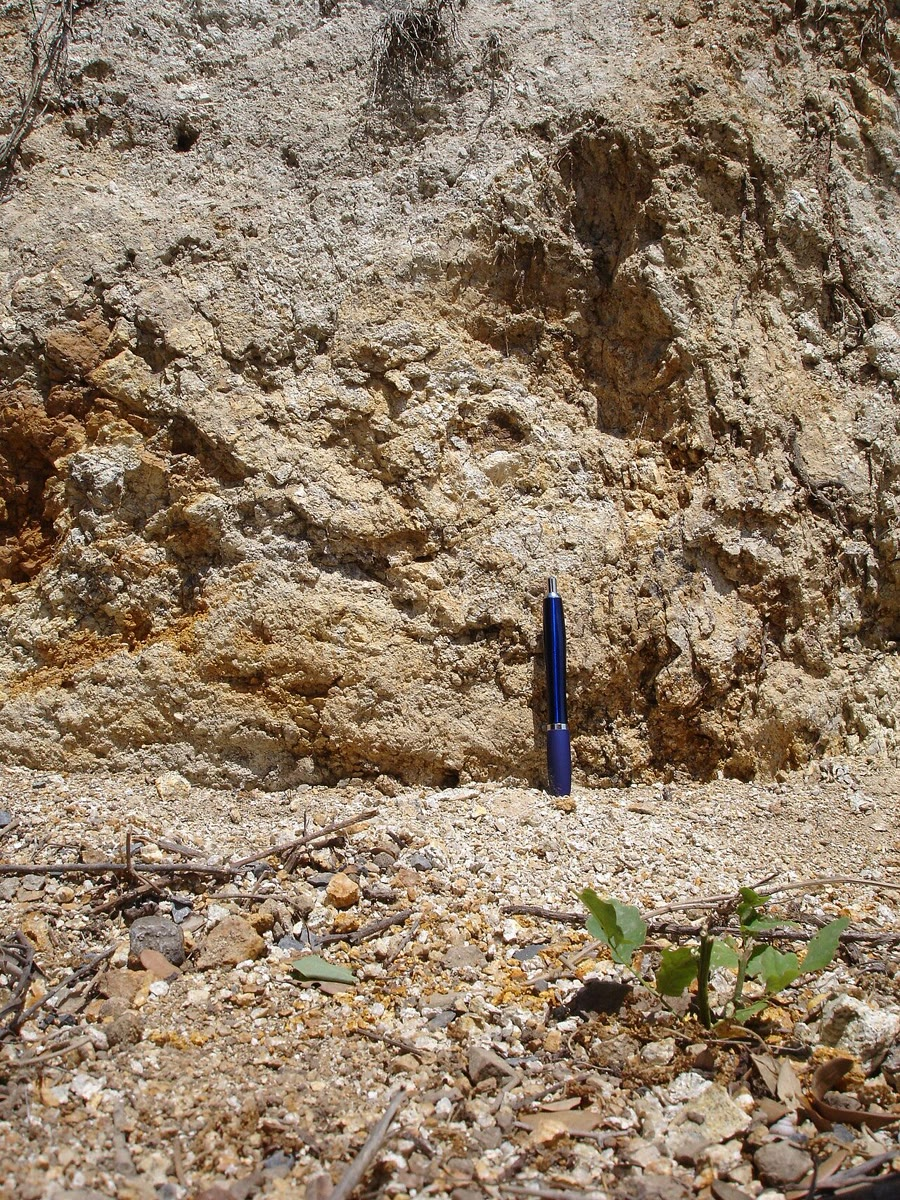
\includegraphics[height=6.3cm]{images/book3/b1-granite-grus.jpg}\hfill
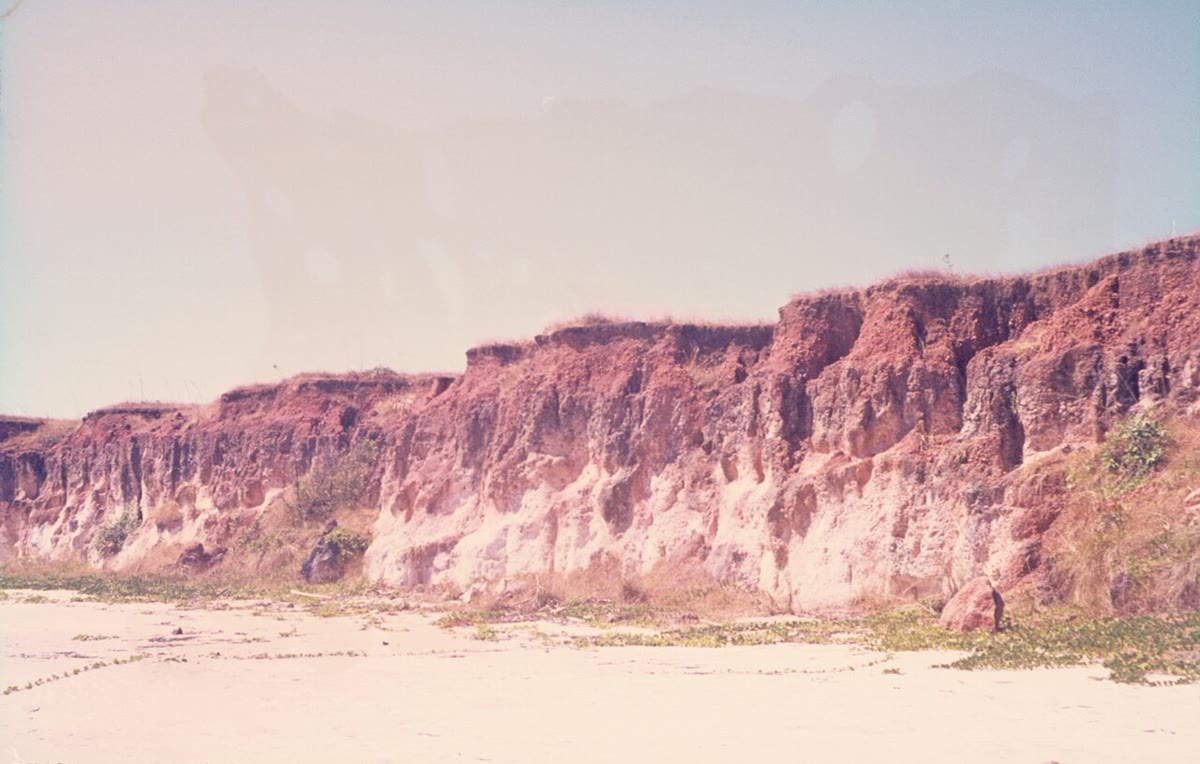
\includegraphics[height=6.3cm]{images/book3/b1-bauxite-weipa.jpg}
\par\smallskip{\small Kiri: granit lapuk di Pyrenees, masih di tempatnya tetapi hancur menjadi pasir kuarsa, \omterm{def:b1:rock-forming-minerals:groups}{feldspar} dan \omterm{def:b1:rock-forming-minerals:groups}{mika}, dengan pasir lepas di kakinya; pena memberi skala. Foto: Pinpin, CC~BY~2.5. Kanan: profil pelapukan di pantai di Weipa, Australia utara: bauksit merah, produk \omterm{def:b1:weathering-clays:hydrolysis-degree}{alitisasi}, di atas batu pasir putih yang kaya \omterm{def:b1:weathering-clays:clay-mineral}{kaolinit}. Foto: Werner Schellmann, 1969, CC~BY-SA~2.5. Keduanya dari Wikimedia Commons.}
\label{fig:b1:weathering-clays:photos}
\end{omfigure}
% ledger: commons:grus, commons:weipa

\emph{\omterm{def:b1:rock-forming-minerals:mineral}{Mineral} mana yang lebih dulu hilang.} Pada 1938 Samuel Goldich, membandingkan profil yang lapuk dengan batuan induknya, mengusulkan deret \omterm{def:b1:rock-forming-minerals:mineral}{mineral} dari yang paling tidak stabil hingga paling stabil dalam pelapukan, dan mendapati bahwa deret itu mengikuti urutan mereka mengkristal dari magma: \omterm{def:b1:rock-forming-minerals:groups}{olivin} dan \omterm{def:b1:rock-forming-minerals:groups}{plagioklas} kaya kalsium lebih dulu, kuarsa terakhir. \omterm{def:b1:rock-forming-minerals:mineral}{Mineral} yang terbentuk pada suhu tertinggi paling jauh dari kesetimbangan di permukaan. Daftar modern, dari yang paling tidak tahan hingga paling tahan, berbunyi: pirit, kalsit, dolomit, \omterm{def:b1:rock-forming-minerals:groups}{olivin}, \omterm{def:b1:rock-forming-minerals:groups}{plagioklas} kaya kalsium, \omterm{def:b1:rock-forming-minerals:groups}{piroksen}, \omterm{def:b1:rock-forming-minerals:groups}{plagioklas} menengah, \omterm{def:b1:rock-forming-minerals:groups}{amfibol}, biotit, \omterm{def:b1:rock-forming-minerals:groups}{feldspar} kalium, muskovit, \omterm{def:b1:weathering-clays:clay-mineral}{smektit}, kuarsa, \omterm{def:b1:weathering-clays:clay-mineral}{kaolinit}, dan oksida gibsit serta hematit. Pengukuran laboratorium tentang laju pelarutan mengonfirmasi peringkat ini; ia tetap berupa peringkat, bukan hukum, karena laju tiap \omterm{def:b1:rock-forming-minerals:mineral}{mineral} juga bergantung pada air di sekitarnya. Produk akhir pelapukan, \omterm{def:b1:weathering-clays:clay-mineral}{kaolinit}, gibsit dan hematit, adalah yang paling tahan dari semuanya: mereka sudah stabil di permukaan.
% ledger: goldich:1938, formoso:weatherability, lasaga:1984

\emph{Neraca massa profil pelapukan.} Pelapukan mengeluarkan materi, sehingga konsentrasi yang diukur pada batuan lapuk tidak menunjukkan berapa banyak yang hilang: hilangnya unsur lain memekatkan unsur yang tinggal. Unsur yang tidak berpindah memberikan acuan.

\begin{proposition}[Neraca massa dengan unsur yang tidak bergerak]\label{prop:b1:weathering-clays:immobile}
Misalkan $i$ adalah unsur yang tidak dipindahkan oleh pelapukan, dengan fraksi massa $C_{i,p}$ pada batuan induk dan $C_{i,w}$ pada batuan lapuk. Maka massa $m_p$ batuan induk menjadi massa $m_w = m_p C_{i,p}/C_{i,w}$ batuan lapuk, dan fraksi unsur lain $j$ yang hilang adalah
\[
  f_j = 1 - \frac{C_{j,w}}{C_{j,p}}\,\frac{C_{i,p}}{C_{i,w}} .
\]
\end{proposition}

\begin{proof}
Massa $i$ kekal: $m_p C_{i,p} = m_w C_{i,w}$, yang memberikan $m_w$.
Massa $j$ berpindah dari $m_p C_{j,p}$ menjadi $m_w C_{j,w}$, sehingga fraksi yang tersisa adalah
$m_w C_{j,w}/(m_p C_{j,p}) = (C_{j,w}/C_{j,p})(C_{i,p}/C_{i,w})$; $f_j$ adalah satu dikurangi fraksi ini.
\end{proof}

Titanium dan zirkonium adalah pilihan yang biasa, dengan alasan yang diberikan oleh bagian berikutnya.

\section{Unsur mana yang keluar: potensial ionik}\label{sec:b1:weathering-clays:ionic}

Natrium, kalium dan kalsium keluar bersama air; aluminium, besi(III) dan titanium tinggal; silikon berada di antaranya. Perbedaannya terletak pada cara setiap ion berperilaku dalam air.

\begin{definition}[Potensial ionik]\label{def:b1:weathering-clays:ionic-potential}
\emph{Potensial ionik}\index{potensial ionik} suatu ion adalah rasio $z/r$ antara bilangan muatannya $z$ dan jari-jari ioniknya $r$, di sini dalam ångström (untuk koordinasi yang sama bagi semua ion, yaitu enam, pada yang berikut).
\end{definition}
% ledger: nomad:goldschmidt, dangic:goldschmidt, shannon:radii-b19

\begin{proposition}[Tiga medan potensial ionik]\label{prop:b1:weathering-clays:fields}
Dalam air pelapukan, ion dengan $z/r < 3$ tetap dalam larutan sebagai kation terhidrasi dan terbawa pergi (kation larut); ion dengan $3 < z/r < 10$ mengikat ion hidroksida dari air dan mengendap sebagai hidroksida atau oksida di tempat mereka dilepaskan (hidrolisat); ion dengan $z/r > 10$ mengikat oksigen begitu kuat sehingga mereka menolak ion hidrogen dan berpindah sebagai oksianion larut, seperti karbonat, sulfat, fosfat dan nitrat. Silikon, pada $z/r = 10$, berada pada batas, dan sebagian terlindi, makin banyak makin intens pelapukannya.
\end{proposition}
\admitted
% ledger: nomad:goldschmidt, dangic:goldschmidt

Aturan ini bersifat empiris, berasal dari Victor Moritz Goldschmidt pada 1930-an, dan batasnya kira-kira; kimia di baliknya, tarik-menarik antara kation dan oksigen molekul air di sekitarnya, termasuk dalam buku-buku kimia. Kation kecil yang bermuatan sangat tinggi menarik elektron molekul airnya begitu kuat sehingga mereka kehilangan ion hidrogen dan menjadi hidroksida: pada tingkat sedang, hidroksida mengendap; pada tingkat ekstrem, bahkan hidroksida pun kehilangan hidrogennya, menyisakan oksianion.

Diagram di bawah ini membaca pelapukan sebuah batuan sekilas pandang. Natrium ($z/r = 0.98$), kalium (0.72), kalsium (2.0) dan magnesium (2.8) keluar: mereka adalah kation air sungai dan air laut. Aluminium (5.6), besi(III) (4.7), titanium (6.6) dan zirkonium (5.6) tinggal, dan menumpuk pada profil yang paling lapuk; titanium dan zirkonium, yang selain itu berada dalam \omterm{def:b1:rock-forming-minerals:mineral}{mineral} yang hampir tidak lapuk, adalah acuan tak bergerak dalam \cref{prop:b1:weathering-clays:immobile}. Silikon (10.0) adalah unsur yang kehilangan sebagiannya menentukan derajat \omterm{def:b1:weathering-clays:hydrolysis}{hidrolisis}.
% ledger: shannon:radii-b19

Oksidasi memindahkan ion melewati batas. Besi(II), dengan $z/r = 2.6$, adalah kation larut; besi(III), pada 4.7, adalah hidrolisat. Dalam tanah yang tergenang air tanpa oksigen, besi larut sebagai \ce{Fe^2+} dan terbawa pergi, menyisakan tanah kelabu; di tempat air bertemu udara, di mata air atau di tanah yang berdrainase baik, besi teroksidasi dan langsung mengendap sebagai oksida merah dan cokelat. Mangan berperilaku dengan cara yang sama, \ce{Mn^2+} (2.4) melawan \ce{Mn^4+} (7.5).
% ledger: nomad:goldschmidt, shannon:radii-b19

\begin{omfigure}
\begin{tikzpicture}[font=\small]
% ionic-potential diagram (figdata/bachelor-1/ionic_potential.py): charge against Shannon radius
\begin{axis}[width=12.5cm, height=8.4cm, xmin=0, xmax=1.8, ymin=0, ymax=7,
    xlabel={jari-jari ionik $r$ (\si{\angstrom}, koordinasi enam)}, ylabel={muatan $z$},
    ytick={1,...,6}, xtick={0,0.2,...,1.8}, xticklabel style={/pgf/number format/fixed},
    axis on top, clip=true]
  \fill[omThm!14] (axis cs:0,0) -- (axis cs:1.8,0) -- (axis cs:1.8,5.4) -- cycle;
  \fill[omDef!16] (axis cs:0,0) -- (axis cs:1.8,5.4) -- (axis cs:1.8,7) -- (axis cs:0.7,7) -- cycle;
  \fill[omExo!18] (axis cs:0,0) -- (axis cs:0.7,7) -- (axis cs:0,7) -- cycle;
  \addplot[black, thick] table[x=r, y=z3] {figdata/out/bachelor-1-ionic_potential-lines.dat};
  \addplot[black, thick] table[x=r, y=z10] {figdata/out/bachelor-1-ionic_potential-lines.dat};
  \addplot[only marks, mark=*, mark size=1.6pt, black,
      point meta=explicit symbolic, nodes near coords,
      visualization depends on={value \thisrow{anc} \as \anc},
      every node near coord/.append style={font=\scriptsize, inner sep=2.6pt, anchor=\anc}]
    table[x=r, y=z, meta=tex] {figdata/out/bachelor-1-ionic_potential-ions.dat};
  \node[font=\footnotesize, align=center, fill=white, fill opacity=0.8, text opacity=1, rounded corners=1pt] at (axis cs:1.45,2.75) {kation larut\\ $z/r < 3$};
  \node[font=\footnotesize, align=center, fill=white, fill opacity=0.8, text opacity=1, rounded corners=1pt] at (axis cs:1.15,6.3) {hidrolisat\\ $3 < z/r < 10$};
  \node[font=\footnotesize, align=left, fill=white, fill opacity=0.8, text opacity=1, rounded corners=1pt, anchor=north west] at (axis cs:0.015,6.95) {oksianion larut, $z/r > 10$};
  \node[font=\scriptsize, rotate=28, anchor=south] at (axis cs:1.62,4.86) {$z/r = 3$};
  \node[font=\scriptsize, rotate=61, anchor=south] at (axis cs:0.2,2.0) {$z/r = 10$};
\end{axis}
\end{tikzpicture}

{\small Diagram \omterm{def:b1:weathering-clays:ionic-potential}{potensial ionik}: setiap ion ditempatkan menurut jari-jari ioniknya yang efektif dalam koordinasi enam (Shannon, 1976) dan muatannya. Garis $z/r = 3$ dan $z/r = 10$ memisahkan ion yang keluar dalam larutan sebagai kation, yang tinggal sebagai hidroksida atau oksida, dan yang keluar sebagai oksianion. Silikon berada pada batas atas.}
\label{fig:b1:weathering-clays:ionic-potential}
\end{omfigure}
% ledger: shannon:radii-b19, nomad:goldschmidt

\section{Mineral lempung}\label{sec:b1:weathering-clays:clays}

\begin{definition}[Mineral lempung, kaolinit, illit, smektit, klorit]\label{def:b1:weathering-clays:clay-mineral}
Sebuah \emph{mineral lempung}\index{mineral lempung} adalah \omterm{def:b1:rock-forming-minerals:silicate-classes}{filosilikat} aluminium terhidrasi, biasanya berbutir beberapa mikrometer atau kurang, tersusun dari lapisan-lapisan yang menggabungkan lembaran tetrahedral (T) dari tetrahedra \ce{SiO4} yang berbagi tiga sudut dan lembaran oktahedral (O) dari aluminium atau magnesium yang dikelilingi oksigen dan hidroksil. Pada \emph{kaolinit}\index{kaolinit}, \ce{Al2Si2O5(OH)4}, setiap lapisan adalah satu lembaran T dan satu lembaran O (lapisan 1:1 atau T--O), tanpa muatan, dan lapisan-lapisannya dipegang oleh ikatan hidrogen. Pada \omterm{def:b1:rock-forming-minerals:mineral}{mineral} lempung 2:1 atau T--O--T, lembaran O terletak di antara dua lembaran T yang mengarah kepadanya: \emph{illit}\index{illit} adalah \omterm{def:b1:rock-forming-minerals:mineral}{mineral} lempung 2:1 yang tidak mengembang, dengan ion kalium di antara lapisan-lapisannya, seperti \omterm{def:b1:rock-forming-minerals:groups}{mika} dengan kalium lebih sedikit; sebuah \emph{smektit}\index{smektit} adalah \omterm{def:b1:rock-forming-minerals:mineral}{mineral} lempung 2:1 dengan kation terhidrasi yang dapat dipertukarkan dan air di antara lapisan-lapisannya, yang dapat menyerap lebih banyak air dan mengembang; sebuah \emph{klorit}\index{klorit} adalah \omterm{def:b1:rock-forming-minerals:mineral}{mineral} 2:1 yang lapisan-lapisannya bermuatan negatif bergantian dengan lembaran oktahedral bermuatan positif bertipe brusit, \ce{(Mg,Fe)(OH)2} dengan sedikit aluminium.
\end{definition}
% ledger: usgs:clay-groups, usgs:clay-settings, webmineral:clays-b19, biscaye:1965

Muatan lapisan menentukan bagaimana lapisan-lapisan itu bertumpuk, dan muatan itu berasal dari substitusi dalam lembaran-lembaran (\cref{def:b1:rock-forming-minerals:substitution}).

\begin{proposition}[Muatan lapisan 2:1]\label{prop:b1:weathering-clays:layer-charge}
Lapisan 2:1 dengan rumus $\mathrm{(Si_{4-x}Al_x)(Al_{2-y}Mg_y)O_{10}(OH)_2}$, dengan $x$ aluminium untuk silikon pada lembaran tetrahedralnya dan $y$ magnesium untuk aluminium pada lembaran oktahedralnya, membawa muatan $-(x + y)$ per satuan rumus.
\end{proposition}

\begin{proof}
Jumlahkan muatannya: $4(4 - x) + 3x$ dari kation tetrahedral, $3(2 - y) + 2y$
dari kation oktahedral, $-2\times10$ dari oksigen dan $-1\times2$ dari
hidroksil: $16 - x + 6 - y - 20 - 2 = -(x + y)$.
\end{proof}

Tanpa substitusi ($x = y = 0$) lapisan itu netral, seperti pada \ce{Al2Si4O10(OH)2}, \omterm{def:b1:rock-forming-minerals:mineral}{mineral} pirofilit, dan lapisan-lapisannya hanya dipegang oleh gaya yang lemah.
Pada muskovit, $x = 1$, muatan $-1$ diseimbangkan oleh satu ion kalium yang mengunci lapisan-lapisannya bersama; \omterm{def:b1:weathering-clays:clay-mineral}{illit} mendekati itu, dengan sedikit lebih sedikit. Pada beidelit dari \cref{prop:b1:weathering-clays:feldspars}, $x = 0.5$: muatan $-0.5$ diseimbangkan oleh $0.5$ natrium. Muatan yang lebih kecil memegang lapisan-lapisannya lebih longgar, dan di antaranya air serta kation terhidrasi dapat masuk: inilah sebabnya \omterm{def:b1:weathering-clays:clay-mineral}{smektit}, dengan muatan sekitar 0.3 hingga 0.5 per satuan rumus, seperti pada rumus montmorilonit dan beidelit, mengembang, sedangkan \omterm{def:b1:weathering-clays:clay-mineral}{illit} tidak.
Kation antarlapisan pada \omterm{def:b1:weathering-clays:clay-mineral}{smektit} dapat dipertukarkan, dan kapasitas tukar kation dari \omterm{def:b1:weathering-clays:clay-mineral}{mineral lempung} yang umum mengikuti strukturnya: 3 hingga 15 miliekuivalen per \qty{100}{g} untuk \omterm{def:b1:weathering-clays:clay-mineral}{kaolinit}, yang lapisannya tidak bermuatan, 10 hingga 40 untuk \omterm{def:b1:weathering-clays:clay-mineral}{illit}, 70 hingga 100 untuk montmorilonit, sebuah \omterm{def:b1:weathering-clays:clay-mineral}{smektit}. Kalium, yang mengunci lapisan-lapisan \omterm{def:b1:rock-forming-minerals:groups}{mika}, mendukung \omterm{def:b1:weathering-clays:clay-mineral}{illit}; \omterm{def:b1:weathering-clays:clay-mineral}{smektit} terbentuk di tempat kalium langka dan kalsium serta magnesium tersedia.
% ledger: webmineral:clays-b19, carroll:cec, usgs:clay-settings

\begin{omfigure}
\begin{tikzpicture}[font=\footnotesize, >={Stealth[length=4pt]}, y=0.2cm, x=1cm]
% schematic clay-mineral structures, vertical scale proportional to the basal spacings
% (USGS OFR 01-041, ledger usgs:clay-xrd): kaolinite 7, illite 10, smectite 14 (air-dried), chlorite 14 angstrom.
% T sheet 2 A thick, O sheet 2.4 A thick (schematic); the column width is 2.2 cm.
\def\W{2.2}
\newcommand{\Tsheet}[1]{% tetrahedral sheet whose base is at y=#1
  \fill[omDef!35] (0,#1) rectangle (\W,#1+2);
  \foreach \i in {0,...,6} {\draw[omDef!80!black, line width=0.4pt] (0.04+\i*0.31,#1) -- (0.195+\i*0.31,#1+2) -- (0.35+\i*0.31,#1) -- cycle;}
}
\newcommand{\TsheetDown}[1]{% inverted tetrahedral sheet, base at the top (y=#1+2)
  \fill[omDef!35] (0,#1) rectangle (\W,#1+2);
  \foreach \i in {0,...,6} {\draw[omDef!80!black, line width=0.4pt] (0.04+\i*0.31,#1+2) -- (0.195+\i*0.31,#1) -- (0.35+\i*0.31,#1+2) -- cycle;}
}
\newcommand{\Osheet}[2]{% octahedral sheet, base at y=#1, fill colour #2
  \fill[#2] (0,#1) rectangle (\W,#1+2.4);
  \foreach \i in {0,...,4} {\draw[black!55, line width=0.4pt] (0.17+\i*0.42,#1+1.2) -- ++(0.17,1.0) -- ++(0.17,-1.0) -- ++(-0.17,-1.0) -- cycle;}
}
\newcommand{\spacing}[3]{% arrow for d001 from y=#1 to y=#2 with label #3
  \draw[<->, line width=0.5pt] (\W+0.18,#1) -- (\W+0.18,#2) node[midway, right, inner sep=2pt] {#3};
  \draw[black!40, densely dotted] (\W,#1) -- (\W+0.28,#1); \draw[black!40, densely dotted] (\W,#2) -- (\W+0.28,#2);
}
% ---------- kaolinite: T-O, d = 7.2
\begin{scope}[xshift=0cm]
  \foreach \b in {0, 7.2} {\Tsheet{\b} \Osheet{\b+2}{omThm!25}}
  \spacing{0}{7.2}{\SI{7}{\angstrom}}
  \node[anchor=north, align=center] at (\W/2,-0.8) {\textbf{kaolinit}\\ lapisan T--O (1:1)\\ dipegang oleh ikatan hidrogen};
\end{scope}
% ---------- illite: T-O-T + K, d = 10
\begin{scope}[xshift=3.6cm]
  \foreach \b in {0, 10} {\Tsheet{\b} \Osheet{\b+2}{omThm!25} \TsheetDown{\b+4.4}}
  \foreach \b in {6.4} {\foreach \i in {0,...,4} \fill[omExo!70!black] (0.25+\i*0.42,\b+1.8) circle[radius=1.5pt];}
  \spacing{0}{10}{\SI{10}{\angstrom}}
  \node[anchor=north, align=center] at (\W/2,-0.8) {\textbf{illit}\\ lapisan T--O--T (2:1)\\ dipegang oleh ion \ce{K+}};
\end{scope}
% ---------- smectite: T-O-T + hydrated cations, d = 14
\begin{scope}[xshift=7.2cm]
  \foreach \b in {0, 14} {\Tsheet{\b} \Osheet{\b+2}{omThm!25} \TsheetDown{\b+4.4}}
  \foreach \i in {0,...,9} {\draw[omDef!60, line width=0.3pt] (0.13+\i*0.215,8.6) circle[radius=1.3pt]; \draw[omDef!60, line width=0.3pt] (0.2+\i*0.215,11.8) circle[radius=1.3pt];}
  \foreach \i in {0,...,3} {\fill[omExo!70!black] (0.35+\i*0.5,10.2) circle[radius=1.5pt];}
  \spacing{0}{14}{\SI{14}{\angstrom}}
  \node[anchor=north, align=center] at (\W/2,-0.8) {\textbf{smektit}\\ lapisan T--O--T, terhidrasi\\ \ce{Na+}, \ce{Ca^2+} dan air};
\end{scope}
% ---------- chlorite: T-O-T + brucite-like O sheet, d = 14
\begin{scope}[xshift=10.8cm]
  \foreach \b in {0, 14} {\Tsheet{\b} \Osheet{\b+2}{omThm!25} \TsheetDown{\b+4.4}}
  \Osheet{9}{omExo!25}
  \spacing{0}{14}{\SI{14}{\angstrom}}
  \node[anchor=north, align=center] at (\W/2,-0.8) {\textbf{klorit}\\ lapisan T--O--T dan\\ lembaran O bertipe brusit};
\end{scope}
% key
\begin{scope}[xshift=0cm, yshift=-2.75cm]
  \fill[omDef!35] (0,0) rectangle (0.4,1.6); \draw[omDef!80!black] (0.05,0) -- (0.2,1.6) -- (0.35,0) -- cycle;
  \node[anchor=west] at (0.5,0.8) {T: lembaran tetrahedral, \ce{SiO4} (sebagian \ce{AlO4})};
  \fill[omExo!70!black] (8.1,0.8) circle[radius=1.5pt]; \node[anchor=west] at (8.3,0.8) {kation antarlapisan};
  \fill[omThm!25] (0,-2.6) rectangle (0.4,-1.0);
  \node[anchor=west] at (0.5,-1.8) {O: lembaran oktahedral, \ce{Al} atau \ce{Mg} dengan \ce{O} dan \ce{OH}};
  \draw[omDef!60] (8.1,-1.8) circle[radius=1.3pt]; \node[anchor=west] at (8.3,-1.8) {molekul air};
\end{scope}
\end{tikzpicture}

{\small Empat famili \omterm{def:b1:weathering-clays:clay-mineral}{mineral lempung} (skematis, dua lapisan masing-masing). Skala vertikal sebanding dengan jarak basal, yaitu jarak ulang dari satu lapisan ke lapisan berikutnya yang diukur dengan difraksi sinar-X: \SI{7}{\angstrom} untuk \omterm{def:b1:weathering-clays:clay-mineral}{kaolinit}, \SI{10}{\angstrom} untuk \omterm{def:b1:weathering-clays:clay-mineral}{illit}, sekitar \SI{14}{\angstrom} untuk \omterm{def:b1:weathering-clays:clay-mineral}{smektit} yang dikeringkan udara dan untuk \omterm{def:b1:weathering-clays:clay-mineral}{klorit}.}
\label{fig:b1:weathering-clays:structures}
\end{omfigure}
% ledger: usgs:clay-xrd, usgs:clay-groups



\begin{table}[htbp]
\centering\footnotesize
\setlength{\tabcolsep}{4pt}
% ledger: usgs:clay-xrd, usgs:clay-groups, usgs:clay-settings, carroll:cec, biscaye:1965
\begin{tabular}{@{}>{\raggedright\arraybackslash}p{1.6cm}>{\raggedright\arraybackslash}p{1.5cm}>{\raggedright\arraybackslash}p{1.6cm}>{\raggedright\arraybackslash}p{1.5cm}>{\raggedright\arraybackslash}p{1.4cm}>{\raggedright\arraybackslash}p{1.4cm}>{\raggedright\arraybackslash}p{1.2cm}>{\raggedright\arraybackslash}p{3.2cm}@{}}
\hline
\omterm{def:b1:rock-forming-minerals:mineral}{mineral} & lapisan & antarlapis & kering udara & glikol & dipanasi & KTK & lingkungan khas \\
\hline
\omterm{def:b1:weathering-clays:clay-mineral}{kaolinit} & T--O & tidak ada & \SI{7}{\angstrom} & \SI{7}{\angstrom} & hancur pada \SI{550}{\celsius} & 3--15 & \omterm{def:b1:rock-forming-minerals:groups}{feldspar} yang tercuci oleh air asam; pelapukan tropis yang intens \\
\omterm{def:b1:weathering-clays:clay-mineral}{illit} & T--O--T & \ce{K+} & \SI{10}{\angstrom} & \SI{10}{\angstrom} & \SI{10}{\angstrom} & 10--40 & air alkalin yang kaya K; dari \omterm{def:b1:rock-forming-minerals:groups}{feldspar} dan \omterm{def:b1:rock-forming-minerals:groups}{mika}; lempung utama batulumpur \\
\omterm{def:b1:weathering-clays:clay-mineral}{smektit} & T--O--T & \ce{Na+}, \ce{Ca^2+} terhidrasi & sekitar \SI{14}{\angstrom} & \SI{17}{\angstrom} & \SI{10}{\angstrom} pada \SI{400}{\celsius} & 70--100 & batuan basa yang lapuk; tanah yang buruk drainasenya, K langka \\
\omterm{def:b1:weathering-clays:clay-mineral}{klorit} & T--O--T & lembaran bertipe brusit & \SI{14}{\angstrom} & \SI{14}{\angstrom} & \SI{14}{\angstrom} & -- & batuan metamorf derajat rendah dan batuan beku yang terubah; batulumpur \\
\hline
\end{tabular}
\caption{Empat famili \omterm{def:b1:weathering-clays:clay-mineral}{mineral lempung}: struktur, jarak basal yang diukur pada preparat terorientasi yang dikeringkan udara, setelah solvasi dengan etilena glikol dan setelah pemanasan, kapasitas tukar kation (KTK, miliekuivalen per \qty{100}{g}; nilai untuk \omterm{def:b1:weathering-clays:clay-mineral}{smektit} adalah nilai montmorilonit) dan tempat mereka biasanya terbentuk.}
\label{tab:b1:weathering-clays:clays}
\end{table}

\begin{inthelab}[Mengidentifikasi mineral lempung dengan difraksi sinar-X]
\omterm{def:b1:weathering-clays:clay-mineral}{Mineral lempung} terlalu halus untuk dibedakan di bawah mikroskop optik. Di laboratorium, fraksi paling halus dari tanah atau batulumpur dipisahkan dengan membiarkan butiran yang lebih kasar mengendap dari air, dan setetes suspensi dikeringkan pada kaca objek, tempat serpihan-serpihannya tergeletak datar: preparat terorientasi. Sinar-X yang dipantulkan oleh lapisan-lapisan bertumpuk memberikan puncak kuat pada sudut-sudut yang ditentukan oleh jarak basal, menurut hukum difraksi Bragg (buku-buku fisika). Preparat dijalankan tiga atau empat kali: dikeringkan udara; setelah semalam dalam uap etilena glikol, yang masuk ke antarlapisan \omterm{def:b1:weathering-clays:clay-mineral}{smektit} dan memekarkannya menjadi \SI{17}{\angstrom} sementara \omterm{def:b1:rock-forming-minerals:mineral}{mineral} lain tidak berubah; setelah dipanaskan hingga \SI{400}{\celsius}, yang mengeluarkan air dari \omterm{def:b1:weathering-clays:clay-mineral}{smektit} dan memampatkannya menjadi \SI{10}{\angstrom}; dan setelah dipanaskan hingga \SI{550}{\celsius}, yang menghancurkan \omterm{def:b1:weathering-clays:clay-mineral}{kaolinit} tetapi menyisakan \omterm{def:b1:weathering-clays:clay-mineral}{illit} dan \omterm{def:b1:weathering-clays:clay-mineral}{klorit}. \Cref{tab:b1:weathering-clays:clays} adalah kunci untuk membaca keempat jalan itu; campuran dan \omterm{def:b1:rock-forming-minerals:mineral}{mineral} berlapis-antar, yang sangat umum dalam tanah, memerlukan lebih banyak.
\end{inthelab}
% ledger: usgs:clay-xrd

\begin{omfigure}
\begin{minipage}[t]{0.66\linewidth}\vspace{0pt}
\emph{Lempung sebagai indikator iklim.} Karena derajat \omterm{def:b1:weathering-clays:hydrolysis}{hidrolisis} mengikuti iklim, \omterm{def:b1:weathering-clays:clay-mineral}{mineral lempung} dari suatu tanah mencatatnya: \omterm{def:b1:weathering-clays:clay-mineral}{kaolinit} dan gibsit di tempat pelapukan intens, di bawah iklim panas dan basah; \omterm{def:b1:weathering-clays:clay-mineral}{smektit} di tempat air sedikit diperbarui; di tempat pelapukan lemah, lempung sebagian besar diwarisi dari batuan, \omterm{def:b1:weathering-clays:clay-mineral}{illit} dan \omterm{def:b1:weathering-clays:clay-mineral}{klorit} dari \omterm{def:b1:rock-forming-minerals:groups}{mika} dan sekis. Sungai membawa lempung ini ke laut, dan endapan lumpur laut dalam menyimpan catatannya: di lepas sungai-sungai kecil Amerika Selatan tropis, yang kaya \omterm{def:b1:weathering-clays:clay-mineral}{kaolinit} dan gibsit, mereka memperlihatkan pelapukan intens dari daratan yang mereka alirkan. Ketika tanah terkubur dan terawetkan, \omterm{def:b1:weathering-clays:clay-mineral}{mineral lempungnya} digunakan untuk menyimpulkan iklim masa geologi lampau: lapisan yang kaya \omterm{def:b1:weathering-clays:clay-mineral}{kaolinit} dalam urutan batulumpur yang kaya \omterm{def:b1:weathering-clays:clay-mineral}{illit} menunjuk pada episode yang hangat dan basah. Inferensi semacam itu memerlukan kehati-hatian, karena \omterm{def:b1:weathering-clays:clay-mineral}{mineral lempung} juga diangkut jauh dari tempat terbentuknya, dan diubah oleh penguburan, \omterm{def:b1:weathering-clays:clay-mineral}{smektit} berubah menjadi \omterm{def:b1:weathering-clays:clay-mineral}{illit} ketika dipanaskan (\cref{ch:b1:diagenesis-basins}).
\end{minipage}\hfill
\begin{minipage}[t]{0.30\linewidth}\vspace{0pt}
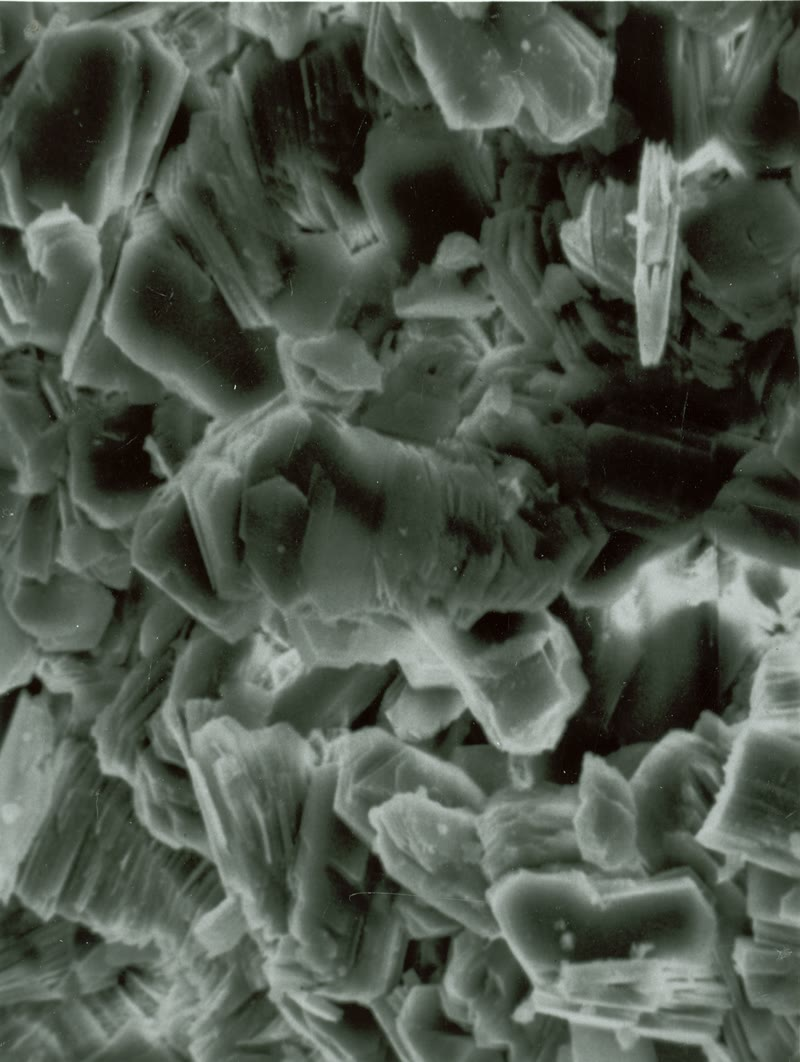
\includegraphics[width=\linewidth]{images/book3/b1-kaolinite-sem.jpg}

{\scriptsize \omterm{def:b1:weathering-clays:clay-mineral}{Kaolinit} yang dilihat dengan mikroskop elektron pemindai: tumpukan keping heksagonal yang berbentuk seperti buku, tumbuh di dalam pori-pori batu pasir di Alaska utara (perbesaran sekitar 1340). U.S. Geological Survey, domain publik, melalui Wikimedia Commons.\par}
\end{minipage}
\end{omfigure}
% ledger: biscaye:1965, usgs:clay-settings, pedron:stages, commons:kaolinite-sem

\emph{\omterm{def:b1:weathering-clays:laterite}{Laterit}.} Di tempat \omterm{def:b1:weathering-clays:hydrolysis}{hidrolisis} mencapai derajat terakhirnya untuk waktu yang lama, profil menebal dan puncaknya memekatkan segala yang tidak keluar.

\begin{definition}[Laterit]\label{def:b1:weathering-clays:laterite}
Sebuah \emph{laterit}\index{laterit} adalah produk kaya besi dan aluminium dari \omterm{def:b1:weathering-clays:hydrolysis}{hidrolisis} yang intens dan berkepanjangan di bawah iklim panas dan basah: bahan merah hingga cokelat, lunak atau mengeras, tersusun dari \omterm{def:b1:weathering-clays:clay-mineral}{kaolinit} dan oksida serta hidroksida besi, dengan gibsit di tempat \omterm{def:b1:weathering-clays:hydrolysis-degree}{alitisasi} tercapai, yang darinya hampir semua kation \omterm{def:b1:rock-forming-minerals:groups}{alkali} dan alkali-tanah serta sebagian besar silika telah dihilangkan.
\end{definition}
% ledger: formoso:laterite, buchanan:laterite

\omterm{def:b1:weathering-clays:laterite}{Laterit} yang cukup kaya gibsit atau boehmit, hidroksida aluminium, adalah bauksit, bijih sembilan persepuluh aluminium: \omterm{def:b1:weathering-clays:hydrolysis-degree}{alitisasi} adalah langkah yang menjadikannya bijih. Kebanyakan bauksit bersifat residual, batuan tempat semua selain alumina telah tercuci; sebagian besar yang tersusun dari gibsit terletak di daerah tropis, dan banyak di antaranya mungkin masih terbentuk.
% ledger: usgs:bauxite

\begin{history}[Sebuah kata dari lapangan]
Pada 1807 Francis Buchanan, yang berkeliling di Malabar, di India selatan, menggambarkan bahan yang penuh rongga dan kaya akan oker merah dan kuning dari besi, tersebar di atas granit dalam massa-massa besar. Ketika digali dari tanah, bahan itu begitu lunak sehingga dapat dipotong dengan pisau, dan penduduk membentuknya menjadi balok; di udara ia segera menjadi keras seperti bata, dan bertahan lebih baik daripada bata mana pun yang pernah ia lihat. Bahasa setempat menyebutnya batu bata; ia mengusulkan nama \omterm{def:b1:weathering-clays:laterite}{laterit}, yang dipertahankan geologi untuk produk merah pelapukan tropis.
\end{history}
% ledger: buchanan:laterite

\section{Pelapukan silikat dan karbon dioksida}\label{sec:b1:weathering-clays:co2}

Ion hidrogen dari \omterm{def:b1:weathering-clays:hydrolysis}{hidrolisis} sebagian besar berasal dari karbon dioksida, sehingga menuliskannya sebagai asam karbonat menunjukkan apa yang dilakukan pelapukan terhadap udara. Untuk kalsium silikat, ditulis \ce{CaSiO3} demi kesederhanaan,
\[
  \ce{CaSiO3 + 2 CO2 + H2O -> Ca^2+ + 2 HCO3- + SiO2},
\]
dan di laut, tempat organisme membangun cangkang kalsium karbonat,
\[
  \ce{Ca^2+ + 2 HCO3- -> CaCO3 + CO2 + H2O}.
\]

\begin{proposition}[Pelapukan dan karbon dioksida]\label{prop:b1:weathering-clays:co2}
(a) Pelapukan silikat mengonsumsi dua mol karbon dioksida, yang diubah menjadi bikarbonat, untuk setiap mol kalsium atau magnesium yang dilepaskan; ketika kalsium atau magnesium diendapkan sebagai karbonat, satu dari dua itu kembali ke udara, dan satu mol tersimpan sebagai batuan karbonat. (b) Pelapukan batuan karbonat dan pengendapan kembali karbonatnya tidak menyimpan apa pun.
\end{proposition}

\begin{proof}
(a) Menjumlahkan kedua persamaan di atas memberikan \ce{CaSiO3 + CO2 -> CaCO3 + SiO2}:
satu \ce{CO2} per kalsium meninggalkan udara untuk selamanya; persamaan pertama saja menunjukkan bahwa dua yang dikonsumsi. Untuk magnesium berlaku hal yang sama, dengan \ce{Mg^2+} menggantikan \ce{Ca^2+}. (b) Pelarutan kalsit, \ce{CaCO3 + CO2 + H2O -> Ca^2+ + 2
HCO3-}, adalah kebalikan persis dari pengendapan: jumlah keduanya nol.
\end{proof}

Dengan \omterm{def:b1:rock-forming-minerals:groups}{feldspar}, asam karbonat menggantikan ion hidrogen dari \cref{prop:b1:weathering-clays:feldspars}: setiap \ce{H+} yang dikonsumsi adalah satu \ce{CO2} yang diubah menjadi \ce{HCO3-}. Anortit dari basal atau gabro dengan demikian mengonsumsi dua mol karbon dioksida per mol sambil berubah menjadi \omterm{def:b1:weathering-clays:clay-mineral}{kaolinit},
\[
  \ce{CaAl2Si2O8 + 2 CO2 + 3 H2O -> Al2Si2O5(OH)4 + Ca^2+ + 2 HCO3-},
\]
dan menyimpan satu dalam jangka panjang. Natrium dan kalium tidak membentuk karbonat di dasar laut, dan penyimpanan jangka panjang dihitung dari kalsium dan magnesium yang dilepaskan.

Sungai membawa bikarbonat ke laut, dan kimia mereka mengukur fluksnya. Dari kimia sungai-sungai besar dunia, karbon dioksida yang dikonsumsi oleh pelapukan silikat benua diperkirakan sebesar \num{11.7e12} hingga \qty{13.6e12}{mol} setahun, sekitar 0.14 hingga 0.16 miliar ton karbon, dari jumlah itu
pelapukan basal saja menyumbang 30 hingga \qty{35}{\percent}. Fluks ini kecil dibandingkan dengan pertukaran karbon antara udara, samudra dan makhluk hidup, tetapi ia tidak berbalik: selama jutaan tahun, ia adalah jalan utama bagi karbon dioksida yang dipasok oleh gunung api untuk keluar dari atmosfer. Karena pelapukan berlangsung lebih cepat ketika lebih hangat dan lebih basah, ia mengikat karbon dioksida udara dengan iklim, yang pada gilirannya bergantung pada karbon dioksida melalui efek rumah kaca: umpan balik negatif yang menstabilkan suhu Bumi sepanjang waktu geologi, dipelajari dalam volume Tahun ke-2.
% ledger: dessert:silicate-co2, whk:1981

\section{Latihan}

\begin{exercise}[$\star$]\label{exo:b1:weathering-clays:1}
Dengan jari-jari \ce{K+} \qty{1.38}{\angstrom}, \ce{Fe^2+} \qty{0.78}{\angstrom},
\ce{Fe^3+} \qty{0.645}{\angstrom} dan \ce{Ti^4+} \qty{0.605}{\angstrom}, hitunglah
\omterm{def:b1:weathering-clays:ionic-potential}{potensial ionik} setiap ion dan sebutkan medannya. Mengapa tanah yang tergenang air kehilangan besinya sedangkan tanah yang berdrainase baik mempertahankannya?
% ledger: shannon:radii-b19
\end{exercise}

\begin{exercise}[$\star$]\label{exo:b1:weathering-clays:2}
Empat fraksi lempung disinar-X sebagai preparat terorientasi. A: puncak pada
\SI{14}{\angstrom}, berpindah ke \SI{17}{\angstrom} oleh etilena glikol dan ke
\SI{10}{\angstrom} oleh pemanasan hingga \SI{400}{\celsius}. B: puncak pada
\SI{7}{\angstrom}, tidak berubah oleh glikol, hilang setelah pemanasan hingga
\SI{550}{\celsius}. C: puncak pada \SI{10}{\angstrom} yang tidak digerakkan oleh perlakuan apa pun. D:
puncak pada \SI{14}{\angstrom} yang tidak digerakkan oleh perlakuan apa pun. Identifikasi setiap \omterm{def:b1:rock-forming-minerals:mineral}{mineral}.
% ledger: usgs:clay-xrd
\end{exercise}

\begin{exercise}[$\star$]\label{exo:b1:weathering-clays:3}
Seimbangkan, dengan \cref{met:b1:weathering-clays:balance}, \omterm{def:b1:weathering-clays:hydrolysis}{hidrolisis} ortoklas \ce{KAlSi3O8} menjadi \omterm{def:b1:weathering-clays:clay-mineral}{kaolinit}. Berapa fraksi kaliumnya dan silikonnya yang keluar dalam larutan?
\end{exercise}

\begin{exercise}[$\star$]\label{exo:b1:weathering-clays:4}
(a) Berapa volume es yang dihasilkan oleh \qty{10}{cm^3} air pada \qty{0}{\celsius}? (b) Dalam kisaran suhu berapakah es yang tumbuh di dalam retakan paling efektif membelah batuan, dan mengapa beku yang lebih ringan maupun yang lebih keras tidak sebaik itu? (c) Sebuah kubus granit bersisi \qty{1}{m} dibelah oleh beku menjadi kubus-kubus bersisi \qty{1}{cm}: dengan faktor berapakah luas permukaannya bertambah?
% ledger: usgs:water-density, iapws:ice-density, wh85:frost
\end{exercise}

\begin{exercise}[$\star\star$]\label{exo:b1:weathering-clays:5}
Hitunglah permukaan spesifik butir \omterm{def:b1:rock-forming-minerals:groups}{feldspar} dengan massa jenis \qty{2600}{kg.m^{-3}}, dianggap sebagai kubus, untuk ukuran \qty{1}{cm}, \qty{1}{mm} dan \qty{1}{\micro m}. Mengapa ukuran butir sangat berpengaruh terhadap laju \omterm{def:b1:weathering-clays:weathering}{pelapukan kimia}, dan mengapa \omterm{def:b1:weathering-clays:weathering}{pelapukan fisik} mempercepat \omterm{def:b1:weathering-clays:weathering}{pelapukan kimia}?
\end{exercise}

\begin{exercise}[$\star\star$]\label{exo:b1:weathering-clays:6}
Satu ton albit \ce{NaAlSi3O8} (\qty{262.22}{g.mol^{-1}}) diubah menjadi \omterm{def:b1:weathering-clays:clay-mineral}{kaolinit} (\qty{258.16}{g.mol^{-1}}). Hitunglah massa \omterm{def:b1:weathering-clays:clay-mineral}{kaolinit} yang terbentuk, massa silika yang diekspor, dihitung sebagai \ce{SiO2} (\qty{60.08}{g.mol^{-1}}), dan massa natrium yang diekspor.
% ledger: webmineral:clays-b19, ciaaw:Na
\end{exercise}

\begin{exercise}[$\star\star$]\label{exo:b1:weathering-clays:7}
Sebuah granit mengandung, menurut massa, \qty{0.30}{\percent} \ce{TiO2}, \qty{3.5}{\percent}
\ce{Na2O}, \qty{72}{\percent} \ce{SiO2} dan \qty{14}{\percent} \ce{Al2O3}; saprolitnya mengandung \qty{0.60}{\percent} \ce{TiO2}, \qty{0.35}{\percent}
\ce{Na2O}, \qty{60}{\percent} \ce{SiO2} dan \qty{27}{\percent} \ce{Al2O3}.
Dengan menganggap titanium tidak bergerak, carilah massa saprolit yang tersisa dari satu kilogram granit dan fraksi natrium, silikon dan aluminium yang hilang. Derajat \omterm{def:b1:weathering-clays:hydrolysis}{hidrolisis} mana yang sedang berlangsung?
\end{exercise}

\begin{exercise}[$\star\star$]\label{exo:b1:weathering-clays:8}
Dengan \cref{prop:b1:weathering-clays:layer-charge}, hitunglah muatan lapisan pirofilit \ce{Al2Si4O10(OH)2}, muskovit \ce{KAl2(Si3Al)O10(OH)2} tanpa kaliumnya, lapisan beidelit \ce{Al2(Si_{3.5}Al_{0.5})O10(OH)2} dan lapisan montmorilonit \ce{(Al_{1.67}Mg_{0.33})Si4O10(OH)2}. Yang manakah dari mereka dapat mengembang, dan mengapa?
% ledger: webmineral:clays-b19
\end{exercise}

\begin{exercise}[$\star\star$]\label{exo:b1:weathering-clays:9}
Forsterit \ce{Mg2SiO4} melapuk menurut
\ce{Mg2SiO4 + 4 CO2 + 4 H2O -> 2 Mg^2+ + 4 HCO3- + H4SiO4}. (a) Periksa persamaannya. (b) Untuk satu ton forsterit, hitunglah karbon dioksida yang dikonsumsi dan karbon dioksida yang disimpan dalam jangka panjang menurut \cref{prop:b1:weathering-clays:co2}. (c) Berapakah hasil perhitungan yang sama untuk satu ton kalsit?
% ledger: ciaaw:Mg, ciaaw:Si, ciaaw:O, ciaaw:C
\end{exercise}

\begin{exercise}[$\star\star\star$]\label{exo:b1:weathering-clays:10}
(a) Di antara jari-jari berapakah ion bermuatan 3 merupakan hidrolisat? (b) Boron,
\ce{B^3+}, memiliki jari-jari \qty{0.27}{\angstrom}: dalam bentuk apakah ia bergerak dalam air? (c) \ce{Mn^2+} memiliki jari-jari \qty{0.83}{\angstrom}, \ce{Mn^4+} \qty{0.53}{\angstrom}. Jelaskan mengapa \omterm{def:b1:layered-earth:layers}{kerak} hitam oksida mangan terbentuk di tempat air mata air, yang miskin oksigen, keluar ke udara. (d) Mengapa silikon tidak dapat sepenuhnya tercuci maupun sepenuhnya dipertahankan?
% ledger: shannon:radii-b19, nomad:goldschmidt
\end{exercise}

\begin{exercise}[$\star\star\star$]\label{exo:b1:weathering-clays:11}
Pelapukan silikat benua mengonsumsi \num{11.7e12} hingga \qty{13.6e12}{mol} karbon dioksida setahun, \qty{4.08e12}{mol} darinya berasal dari basal. (a) Ubahlah rentang itu menjadi ton karbon dan ton karbon dioksida setahun. (b) Berapa bagian yang diambil basal? (c) Jika semua ini berasal dari silikat kalsium dan magnesium, berapa banyak karbon yang akan tersimpan dalam jangka panjang setiap tahun? Mengapa angka jangka panjang yang nyata lebih kecil?
% ledger: dessert:silicate-co2, ciaaw:C, ciaaw:O
\end{exercise}

\begin{exercise}[$\star\star\star$]\label{exo:b1:weathering-clays:12}
Tiga fraksi lempung, yang telah dibebaskan dari kuarsa dan oksida besi, dianalisis (persen
massa): A, \ce{SiO2} \num{46.55} dan \ce{Al2O3} \num{39.50}; B, \ce{SiO2} 60 dan
\ce{Al2O3} 25; C, \ce{SiO2} 2 dan \ce{Al2O3} 63 (\ce{SiO2}
\qty{60.08}{g.mol^{-1}}, \ce{Al2O3} \qty{101.96}{g.mol^{-1}}). Hitunglah rasio molar Si/Al masing-masing, sebutkan derajat \omterm{def:b1:weathering-clays:hydrolysis}{hidrolisis} yang dicatatnya, dan letakkan ketiga tanah itu pada satu garis dari pencucian paling sedikit hingga paling intens.
% ledger: webmineral:clays-b19, pedron:stages, formoso:laterite
\end{exercise}

\section{Masalah: dari granit ke lempung}

\begin{problem}[{Soal akhir pekan --- feldspar granit dan gabro, dari reaksi yang seimbang
hingga karbon dioksida yang dibawa sungai}]
\label{pb:b1:weathering-clays:1}
% values: calc/ch19.py; the river is invented (its numbers are of a realistic order)
Kedua \omterm{def:b1:rock-forming-minerals:groups}{feldspar} itu adalah albit \ce{NaAlSi3O8} (\qty{262.22}{g.mol^{-1}}, massa jenis
\qty{2.62}{g.cm^{-3}}) dan anortit \ce{CaAl2Si2O8}
(\qty{278.20}{g.mol^{-1}}, massa jenis \qty{2.75}{g.cm^{-3}}). \omterm{def:b1:weathering-clays:clay-mineral}{Kaolinit}
\ce{Al2Si2O5(OH)4} memiliki massa molar \qty{258.16}{g.mol^{-1}} dan massa jenis
\qty{2.6}{g.cm^{-3}}; gibsit \ce{Al(OH)3}, \qty{78.00}{g.mol^{-1}}. Gunakan
\ce{SiO2} \qty{60.08}{g.mol^{-1}}, \ce{CO2} \qty{44.01}{g.mol^{-1}}, \ce{HCO3-}
\qty{61.02}{g.mol^{-1}}, Na \num{22.99} dan Ca \qty{40.08}{g.mol^{-1}}.
% ledger: hom:albite, hom:anorthite, webmineral:clays-b19, ciaaw:Na, ciaaw:Ca, ciaaw:C, ciaaw:O, ciaaw:H

\medskip
\noindent\textbf{Bagian I --- Reaksinya.}
\begin{enumerate}
  \item Seimbangkan \omterm{def:b1:weathering-clays:hydrolysis}{hidrolisis} albit menjadi \omterm{def:b1:weathering-clays:clay-mineral}{kaolinit}.
  \item Seimbangkan \omterm{def:b1:weathering-clays:hydrolysis}{hidrolisis} anortit menjadi \omterm{def:b1:weathering-clays:clay-mineral}{kaolinit}. Apa yang istimewa darinya?
  \item Seimbangkan \omterm{def:b1:weathering-clays:hydrolysis}{hidrolisis} anortit menjadi gibsit.
  \item Seimbangkan \omterm{def:b1:weathering-clays:hydrolysis}{hidrolisis} albit menjadi beidelit
        \ce{Na_{0.5}Al2(Si_{3.5}Al_{0.5})O10(OH)2}, dan periksa hidrogennya.
  \item Tuliskan ulang dua reaksi pertama dengan asam karbonat sebagai sumber
        ion hidrogen: \ce{CO2 + H2O -> H+ + HCO3-}.
  \item Manakah dari reaksi-reaksi ini yang merupakan \omterm{def:b1:weathering-clays:hydrolysis-degree}{bisiallitisasi}, \omterm{def:b1:weathering-clays:hydrolysis-degree}{monosiallitisasi} dan \omterm{def:b1:weathering-clays:hydrolysis-degree}{alitisasi}?
\end{enumerate}

\medskip
\noindent\textbf{Bagian II --- Apa yang tinggal, apa yang keluar.}
\begin{enumerate}[resume]
  \item Berapa mol yang ada dalam satu ton albit, dan dalam satu ton anortit?
  \item Hitunglah massa \omterm{def:b1:weathering-clays:clay-mineral}{kaolinit} yang terbentuk dari satu ton masing-masing.
  \item Hitunglah massa silika (sebagai \ce{SiO2}), natrium dan kalsium yang diekspor dalam larutan.
  \item Hitunglah volume satu ton masing-masing \omterm{def:b1:rock-forming-minerals:groups}{feldspar} dan \omterm{def:b1:weathering-clays:clay-mineral}{kaolinit} yang dihasilkannya. Berapa fraksi volume padatan menyusut?
  \item Saprolit mempertahankan bentuk batuan yang digantikannya. Apa yang mengisi ruang yang tersisa dalam granit lapuk yang kaya albit? Mengapa gabro lapuk yang kaya anortit tetap lebih padat?
  \item Dengan diagram \omterm{def:b1:weathering-clays:ionic-potential}{potensial ionik}, jelaskan unsur-unsur dari kedua \omterm{def:b1:rock-forming-minerals:groups}{feldspar} mana yang keluar dan mana yang tinggal.
\end{enumerate}

\medskip
\noindent\textbf{Bagian III --- Karbon dioksida.}
\begin{enumerate}[resume]
  \item Berapa mol, dan berapa kilogram, karbon dioksida yang dikonsumsi ketika satu ton albit berubah menjadi \omterm{def:b1:weathering-clays:clay-mineral}{kaolinit}?
  \item Pertanyaan yang sama untuk satu ton anortit.
  \item Berapa massa bikarbonat yang diekspor oleh anortit?
  \item Apa yang terjadi pada bikarbonat ini di laut? Berapa banyak karbon dioksida yang dikonsumsi kembali ke udara?
  \item Mengapa tidak ada penyimpanan jangka panjang yang dihitung untuk natrium dari albit?
  \item Bandingkan dengan pelarutan satu ton kalsit yang diikuti oleh pengendapannya.
\end{enumerate}

\medskip
\noindent\textbf{Bagian IV --- Sebuah sungai.}
\begin{enumerate}[resume]
  \item Sebuah sungai mengalirkan \qty{50000}{km^2} granit dan gneis, dengan debit rata-rata \qty{200}{m^3.s^{-1}}; bikarbonat yang dibawanya dari pelapukan silikat adalah \qty{0.3}{mmol.L^{-1}}. Hitunglah fluks tahunan bikarbonat ini, dalam mol, dan per kilometer persegi.
  \item Nyatakan itu sebagai mol anortit yang pelapukannya menjadi \omterm{def:b1:weathering-clays:clay-mineral}{kaolinit} akan memasoknya, lalu sebagai ton anortit setahun dan per kilometer persegi.
  \item Jika batuan mengandung setara \qty{20}{\percent} anortit dan memiliki massa jenis \qty{2700}{kg.m^{-3}}, dengan laju berapa, dalam meter per juta tahun, batuan segar itu sedang terkikis?
  \item Berapa banyak karbon dioksida yang dikeluarkan sungai ini dari udara untuk selamanya setiap tahun?
  \item Mengapa laju pada soal 21 merupakan batas bawah bagi penurunan permukaan daratan?
  \item Dalam kilogram, dengan tiga angka penting, berapa banyak karbon dioksida yang ditarik untuk selamanya oleh pelapukan satu ton anortit?
\end{enumerate}
\end{problem}
